
\section{Background}
This section motivates \sys in relation to prior work.
Using the pilot study as inspiration, we use a simplified running example to present the system and notation:
\begin{example}[Lead Prediction]\sloppy\label{ex:lead}
Past clients are stored in a relational database:
\[
R(id, name, num\_emp, industry, region, successful)
\]
where $name$ is the company name, $num\_emp$ is the number of employees in the company, $industry$ is a categorical attribute that describes the industry segment, $region$ is a code indicating the region of the country the business is headquartered, and $is\_successful$ is a Boolean describing whether the company purchased the product.
\end{example}

\begin{figure}[t]
% \vspace{-5pt}
\centering
 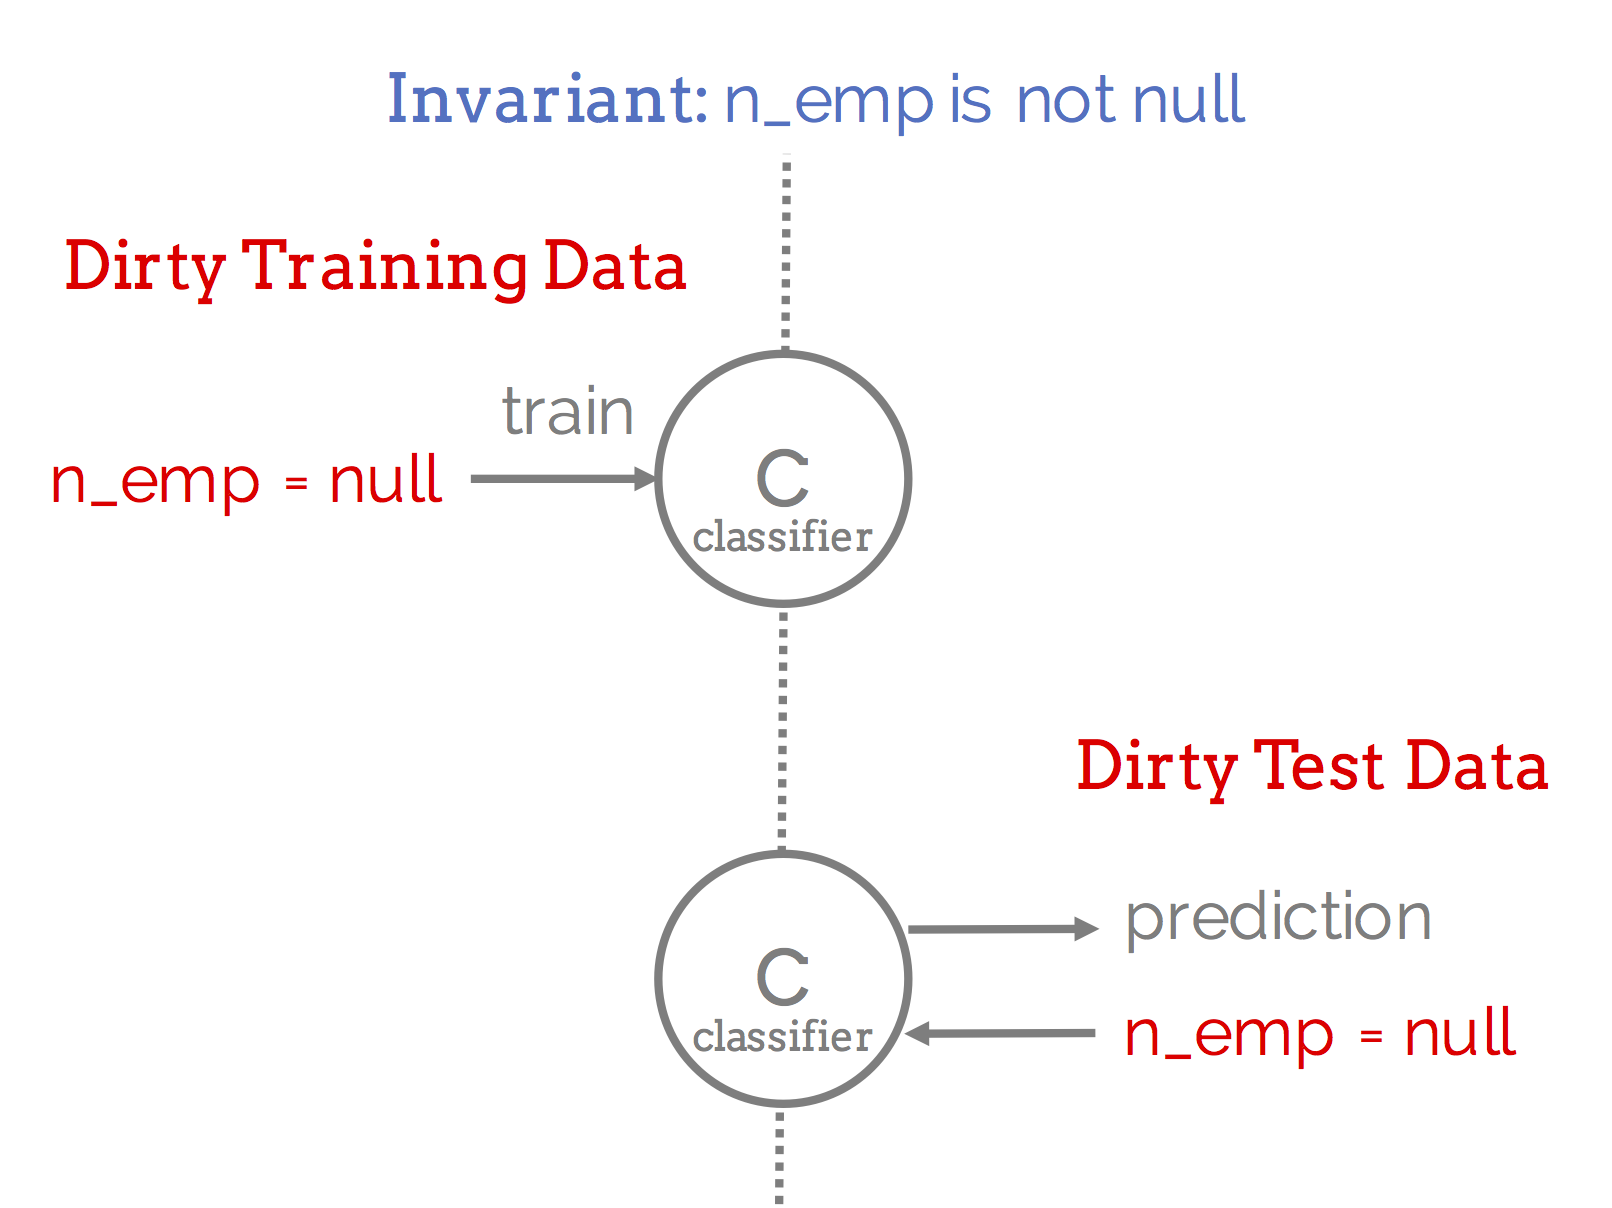
\includegraphics[width=\columnwidth]{figures/training_and_pred_errors.png}
 \caption{The above example uses the invariant that the number of employees is greater than $0$.  Training errors are violations of the invariant in the training dataset (top row). Prediction errors are invariant violations in the test data during prediction. \sys is a tool to {\it detect} both types of errors and generate a corrective {\it repair} action.
 \label{fig:error}}
\end{figure}

\subsection{Machine Learning and Dirty Data}
We feel it is important to highlight a number of points when considering data cleaning in the machine learning context.
First, machine learning models are often robust to statistical noise and inherent variations in the dataset.  For this reason, our focus is not to reduce random noise; instead, our focus is to identify and address systematic errors due to invariant violations that lead to unforeseen biases in the model.  
For example, records with a positive classification label are more likely to have NULL values in the training set.
Second, while the notion of invariants is similar to integrity constraints in traditional relational data cleaning, the way that repairs are evaluated differ.  Relational data cleaning focuses on identifying a minimal set of repairs that resolve a set of constraint violations.  On the other hand, our goal is to improve the the downstream model test prediction accuracy.  These goals are not necessarily aligned, and by ignoring the downstream model, it is possible that traditional cleaning techniques perform cleaning operations that degrade the model accuracy.
Finally, acquiring a clean dataset to evaluate traditional data cleaning algorithms~\cite{DBLP:journals/pvldb/AbedjanCDFIOPST16} is often challenging or impossible.  In contrast, test data is already available in data science applications, and our research explores how this data can be leveraged to identify and repair data errors.

\subsection{Existing Approaches}
\sys brings together generic, dataset-independent error detection with automatically learned repair strategies for ML applications.
We review how baseline techniques proposed in prior work that could apply to this problem.

\vspace{0.5em}

\noindent\textbf{Rule-based Repair: } 
The traditional relational approach is to directly, and completely clean the relation.
In the running example, suppose some of the values for $num\_emp$ are NULL and we want to train a classifier to predict $is\_successful$.
We would define a domain integrity constraint $num\_emp \ne~NULL$, and then propose a set of repairs to satisfy this constraint.
With no other information, this rule-based approach could in principle impute any non-null value from the domain to create a logically consistent relation.
To avoid this problem, we can adopt an approach like~\cite{prokoshyna2015combining} and select the imputations that minimize the statistical distance of the updated relation to an ideal distribution for the attribute, for example, an ideal power-law distribution.
This would impute values in such a way that $num\_emp$ matched a Zipfian distribution.

When we train a classifier after applying such a technique, counter-intuitive effects can occur.  
The data cleaning operation may break important correlations in the data and may introduce biases into the training data not present in test conditions. 
Consider the degenerate case where $num\_emp = NULL$ is perfectly correlated with one of the prediction classes--in this case, it may be better to NOT clean the data!
While more sophisticated statistical imputation techniques exist~\cite{schafer1998multiple}, they all have the same fundamental problem that the value imputation is divorced from the downstream classifier's predictive accuracy. 
We see this problem in our experiments (Section~\ref{exp:comp}), where on some datasets imputing the most frequent value leads to a more accurate downstream classifier than imputing to minimize the difference from an ideal distribution.

\vspace{0.5em}\noindent\textbf{Statistical Detection: } Rule-based techniques are dependent on the analyst defining the invariants. Defining such invariants can be challenging if the analyst is working with a new dataset, if she cannot anticipate how future data might look, or if the number of datasets is too large (e.g., in a data lake setting).
There is a well-established line of literature on statistical anomaly detection~\cite{hellerstein2008quantitative}, and for the most part, these techniques are generic and dataset independent (up-to hyperparameters). Typically, such approaches identify \emph{outlier} records outside of some normal range of variance. However, the problem is that not all dirty data look like outliers. In the running example, there could truly be companies where $num\_emp = 0$. It has been shown that statistical anomaly detection techniques miss obvious errors in heterogeneous datasets that contain a mixture numerical, categorical, and string-valued attributes~\cite{DBLP:journals/pvldb/AbedjanCDFIOPST16}.

Abedjan et al. recently evaluated a wide range of error detection techniques on 5 proprietary real-world datasets~\cite{DBLP:journals/pvldb/AbedjanCDFIOPST16}.  They found that the errors in 3 of the datasets were dominated by missing cell values; 1 dataset contained functional dependency violations due to erroneous numerical attribute values, and only 1 dataset require complex user-specified denial constraints~\cite{chu2013discovering} to identify the errors.  These findings suggest that, in 4 of the 5 datasets, a significant portion of data errors can be classified as {\it domain integrity errors}, wherein a cell contains a value outside of its domain of permissible values.

\stitle{Towards Automated Cleaning:} We believe this highlights the potential value of automated cleaning systems such as \sys to identify the bulk of common-case errors, so that developers may focus on the specialized, domain-specific errors.  The prevalence of {\it domain integrity errors} suggests that a pre-defined set of featurizers and detector generators can be sufficient to detect these errors.  In fact, on 8 of our experimental datasets, \sys using our pre-populated detector library achieves a detection accuracy of 81\% of all of the errors found by hand-written rules.

Therefore, we need a mix of statistical rules and logic rules to determine errors.
We explore to what extent we can derive these rules from data for routine errors. 
We surveyed 8 ML datasets used in Kaggle competitions and benchmarks in the UCI ML repository, and found that a majority of the non-statistical errors could be detected as \emph{domain integrity constraints}, i.e., disallowed values in single columns.
We apply a combination of heuristic checks for missing values and data type errors, and a neural network based error detector that identifies attribute values not likely to co-occur in the same record.

\iffalse
\subsection{Solution Overview}
There does not exist one single error detector or repair action that dominates, so which ones should an analyst choose? 
\sys models this problem as a boosting problem.
Rather than thinking of each of detector and repair pair as a data transformation, it thinks of each as generating a new ``classifier'' that provides some additional information about the label.
The problem of selecting the top data pairs is equivalent to ensembling a subset of the classifiers as best as possible.
We choose a boosting framework to represent this problem due to the relatively minimal assumptions about the structure and implementation details of the user-specified classifier.
To construct the underlying library of cleaning operations we surveyed datasets on Kaggle and the UCI repository and built a library of data cleaning operations that supported common data cleaning tasks across the datasets.
\fi